\documentclass[12pt]{article}

\usepackage[margin=50pt]{geometry}
\usepackage{amsmath}
\usepackage{amssymb}
\usepackage{graphicx}
\usepackage{array}
\usepackage{multicol}
\usepackage{qtree}
\usepackage{blkarray}
\usepackage{hyperref}

\graphicspath{/images}
\geometry{footskip=0.8cm}

\newlength{\Oldarrayrulewidth}
\newcommand{\Cline}[2]{%
  \noalign{\global\setlength{\Oldarrayrulewidth}{\arrayrulewidth}}%
  \noalign{\global\setlength{\arrayrulewidth}{#1}}\cline{#2}%
  \noalign{\global\setlength{\arrayrulewidth}{\Oldarrayrulewidth}}
}

\newcommand\Thickvrule[1]{%
  \multicolumn{1}{!{\vrule width 2pt}c!{\vrule width 2pt}}{#1}%
}

\title{Dynamic Game Theory}
\author{Thomas Vroom}

\begin{document}
\maketitle

\tableofcontents

%
% Topic 1 - Games in Normal Form
%
\newpage
\section{Games in Normal Form}
A game in \textbf{normal form} is defined by a triple $\left\langle S, \left(A^k\right)_{k \in S}, \left(r^k\right)_{k \in S} \right\rangle$, where $S = \{ 0, 1, 2, ... , n \}$ is the set of players, $A^k$ is the set of strategies for player $k$ and $r^k : A^k \rightarrow \mathbb{R}$ is the payoff function for player $k$.
Using the \textbf{rationality} assumption we can assume that each player knows the set of players, all possible actions each player can choose and the possible payoffs for each combination of actions.
We also assume that each player wants to maximize their individual payoff, and knows their opponents want to maximize their individual payoff.
All players are assumed to choose their actions simultaneously and independent of each other.

\noindent
\\
In this chapter we will illustrate these concepts by looking at two-player normal form games, also called \textbf{bimatrix games}.
These games can be represented by a matrix with two numbers in each entry.
It is usual to have the rows correspond to the strategies of player 1, while the columns correspond to the strategies of player 2 (in the context of bimatrix games, strategies are often called \textbf{actions}).
A bimatrix game in which players 1 and 2 respectively have $m$ and $n$ actions can be represented by a matrix of the form:

\[ (A, B) = [a_{ij}, b_{ij}] = \begin{pmatrix}
    a_{11}, b_{11} & a_{12}, b_{12} & \dots & a_{1j}, b_{1j} & \dots & a_{1n}, b_{1n} \\
    a_{21}, b_{21} & a_{22}, b_{22} & \dots & a_{2j}, b_{2j} & \dots & a_{2n}, b_{2n} \\
    \vdots & \vdots & & \vdots & & \vdots \\
    a_{i1}, b_{i1} & a_{i2}, b_{i2} & \dots & a_{ij}, b_{ij} & \dots & a_{in}, b_{in} \\
    \vdots & \vdots & & \vdots & & \vdots \\
    a_{m1}, b_{m1} & a_{m2}, b_{m2} & \dots & a_{mj}, b_{mj} & \dots & a_{mn}, b_{mn}
\end{pmatrix} \]

\subsection{Nash-Equilibrium}
Player 1 would like to choose row $i$ to maximize their payoff $a_{i\dots}$, while player 2 would like to choose column $j$ to maximize their payoff $b_{\dots j}$.
Their final payoff will of course also be dependent on the choice of the other player.
This means both players are looking for the \textbf{best replies} to the other player's choice.
Player 1 would like to have chosen some $i^*$ in such a way that, against $j^*$ chosen by player 2, they could not have done any better:
\[ a_{i^* j^*} = \max_i a_{ij^*} \]

\noindent
Clearly, player 2 would also want their action $j^*$ to be the best reply to $i^*$:

\[ b_{i^* j^*} = \max_j a_{i^*j} \]

\noindent
A pair of actions / strategies that are best replies against each other is called a \textbf{Nash-equilibrium}.
Take a look at the following bimatrix game:

\[ \begin{pmatrix}
    2,1 & 0,0 \\
    0,0 & 1,2
\end{pmatrix} \]

\noindent
This game has two equilibria: $(T, L)$ and $(B, R)$.
Note that the payoffs of these equilibria are not the same; player 1 would prefer to play $(T, L)$, but player 2 would prefer to play $(B, R)$.
This shows that the payoffs of a Nash-equilibrium are not necessarily optimal for both players.

\newpage
\noindent
Consider the same bimatrix game, but now with the following payoffs:

\[ \begin{pmatrix}
    2,0 & 0,2 \\
    0,1 & 1,0
\end{pmatrix} \]

\noindent
We can quickly observe that there is no pair of actions $(i^*, j^*)$ that are best replies to each other in this game.
Let's imagine that in this example player 2 has somehow found out what player 1 is going to do, then clearly player 1 will end up only getting 0.
Player 1 could of course anticipate player 2's behavior, but then we would quickly find ourselves in an infinite loop.

\noindent
\\
A better way for player 1 to camouflage their intention would be to choose their action randomly (e.g. flipping a coin to decide if they are going to pick $T$ or $B$).
If player 2 finds out about this plan they need to evaluate what is best for them:

\begin{enumerate}
    \item If player 2 chooses $L$, then with probability $\frac{1}{2}$ they will receive 0 and with probability $\frac{1}{2}$ they will receive 1.
    This means player 2's \textbf{expected payoff} for choosing $L$ is $\frac{1}{2} \cdot 0 + \frac{1}{2} \cdot 1 = \frac{1}{2}$.
    \item If player 2 chooses $R$, then with probability $\frac{1}{2}$ they will receive 2 and with probability $\frac{1}{2}$ they will receive 0.
    This means player 2's \textbf{expected payoff} for choosing $R$ is $\frac{1}{2} \cdot 2 + \frac{1}{2} \cdot 0 = 1$.
\end{enumerate}

\noindent
Assuming player 1 decides their choice using a coin flip, it seems better for player 2 to choose $R$.
Using probability devices, player 1 could choose any action with any probability they like.
This drastically increases player 1's set of possible actions.
We call these probabilistic actions \textbf{mixed actions}.
For player 1, a mixed action in an $m \times n$-bimatrix game is a vector $(p_1, p_2, ... , p_m)$, where $p_i \geq 0$ is the probability of choosing action $i$, and $p_1 + p_2 + ... + p_m = 1$.

\subsection{Best Reply Functions}
For two-player games, a structural approach to find strategies that are best replies to each other is by drawing a diagram of the \textbf{best reply functions}:
\[ B_1(q) = \{ x \in (0, 1) : (1 - x, x) \text{ is a best reply for player 1 against } (1 - q, q) \} \]
\[ B_2(p) = \{ y \in (0, 1) : (1 - y, y) \text{ is a best reply for player 2 against } (1 - p, p) \} \]

\noindent
With $p, q \in (0, 1)$ for player 2 and 1 respectively.

\begin{figure}[h!]
    \centering
    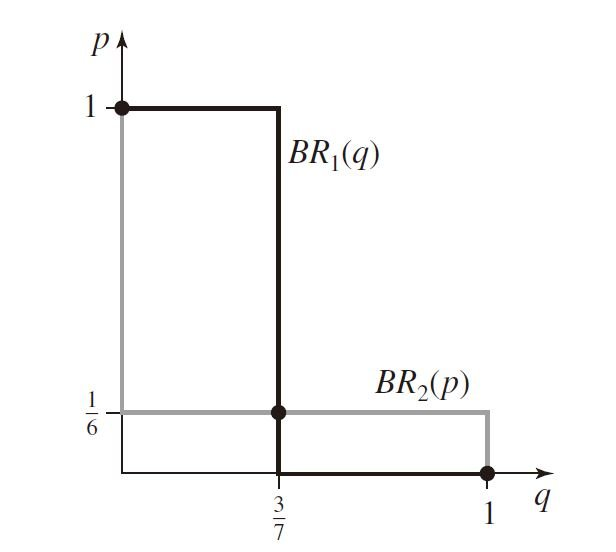
\includegraphics[scale=0.49]{images/bestreplydiagram.png}
    \caption{An example of a \textbf{best reply diagram} with 3 equilibria.}
\end{figure}

\newpage
\noindent
It has been shown that any $n$-player game, in which each player has finitely many actions, has at least one Nash-equilibrium in mixed actions.
If there is more than one, it is important to realize that the payoffs of these equilibria may be very different from each other.
For example, if the players in the bimatrix game mentioned at the start of this chapter want to play the mixed equilibrium:

\[ \left( \left( \frac{2}{3},\frac{1}{3} \right) , \left( \frac{1}{3},\frac{2}{3} \right) \right) \]

\noindent
Then with probability $\frac{2}{9}$ this would lead to the players ending up in the situation $(T, L)$ with payoffs $(2, 1)$; with probability $\frac{2}{9}$ it would yield the situation $(B, R)$ with payoffs $(1, 2)$; but also, with probability $\frac{5}{9}$ play would end in one of the entries with payoffs $(0, 0)$.
The expected payoff for the players would be:
\[ \frac{2}{9} \cdot (2, 1) + \frac{2}{9} \cdot (1, 2) + \frac{5}{9} \cdot (0, 0) = \left( \frac{6}{9},\frac{6}{9} \right) \]

\noindent
In expected payoff it is important to realize that, assuming the players are independently trying to maximize their individual payoff, receiving a payoff of $1\,000\,000$ with probability $\frac{1}{2}$ or losing $1\,000\,000$ with probability $\frac{1}{2}$ is worth just as much as receiving a payoff of 0.
Of course, in real life not everyone would like to take the risk of having to pay $1\,000\,000$, but in game theory we assume that the players are \textbf{risk neutral}.

\subsection{Dominated Strategies}
A famous bimatrix game is the \textbf{Prisoner's Dilemma}:
\[ \begin{pmatrix}
    3,3 & 0,5 \\
    5,0 & 1,1
\end{pmatrix} \]

\noindent
In this game we can observe that for player 1 playing $B$ is strictly better than playing $T$.
No matter what action player 2 chooses, playing $B$ will always yield a higher payoff for player 1.
We say that the action $T$ is \textbf{dominated} by playing $B$.
Similarly, we can say that the action $L$ is dominated by the action $R$ for player 2.
Clearly in any equilibrium none of the players is going to play a dominated strategy.
This means that we can remove the dominated strategies from the game without changing the set of equilibria.

%
% Topic 2 - Matrix Games
%
\newpage
\section{Matrix Games}
In this section we will examine a special type of games in normal form: \textbf{matrix games}.
These are bimatrix games $(A, B)$ for which $B = -A$.
This means that for any choice $i, j$ of player 1 and 2 we have $b_{ij} = -a_{ij}$.
These games are often called \textbf{zero-sum games}, since the sum of the payoffs for the players is always 0.
For a matrix game we immediately know the payoffs for player 2 as soon as we know the payoffs for player 1.
Therefore, we can represent a matrix game by just giving the matrix $A$ of payoffs for player 1.
The assumption that player 2 is trying to maximize their own payoff is the same as the assumption that player 2 is trying to minimize player 1's payoff.

\subsection{Saddle Points}
Take the following matrix game:

\[ A = \begin{pmatrix}
    -3 & 5 \\
    0 & 1
\end{pmatrix} \]

\noindent
For player 2, the action $R$ is being dominated by the action $L$, meaning that player 2 will always play $L$.
Player 1, knowing this, will always play $B$ to maximize their payoff.
This means that the strategy $(B, L)$ is a Nash-equilibrium.

\noindent
\\
If a matrix game has an equilibrium in pure actions $(i^*, j^*)$, then we call this equilibrium a \textbf{saddle point}.
This means that, by definition, the related payoff is the maximum of column $j^*$ and at the same time the minimum of row $i^*$:
\[ a_{i^* j} \geq a_{i^* j^*} \geq a_{i j^*} \]

\noindent
We could also write this expression as:
\[ \min_{j} a_{i^* j} = a_{i^* j^*} = \max_{i} a_{i j^*} \]

\noindent
Through some rewriting, we can find the following equivalent statement:
\[ \max_{i} \min_{j} a_{ij} = a_{i^* j^*} = \min_{j} \max_{i} a_{ij} \]

\noindent
This means that the payoff of a saddle point equals the \textbf{largest row minimum} and the \textbf{smallest column maximum}.
Conversely, if the largest row minimum equals the smallest column maximum, then there exists at least one saddle point.

\subsection{The Minimax-Theorem}
Take a look at the following matrix game:

\[ A = \begin{pmatrix}
    0 & -2 & 5 \\
    4 & 10 & -1
\end{pmatrix} \]

\noindent
We can find the largest row minimum $\max_{i} \min_{j} a_{ij} = -1$ and the smallest column maximum $\min_{j} \max_{i} a_{ij} = 4$.
Therefore, by playing pure actions, player 1 can be sure of getting at least -1, while player 2 can be sure of paying at most 4.
However, these points are not equilibria, as the opposing player could play better moves in each situation.
Like in bimatrix games, the players might be able to guarantee a better payoff by playing mixed actions.

\newpage
\noindent
For player 1 a mixed action can be given as $(1 - p, p)$, where $p \in (0, 1)$ is the probability of playing $B$.
Let $f_j(p)$ denote the expected payoff for player 1 if they play $(1 - p, p)$, while player 2 plays column $j$.
We can visualize these functions in the following plot:

\begin{figure}[h]
    \centering
    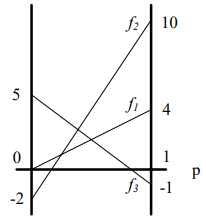
\includegraphics{images/f123plot.PNG}
\end{figure}

\noindent
Player 1 wants to maximize their minimum (expected) payoff, which can be visualized as the function $f_-(p) = \min \{ f_j(p) \}$:

\begin{figure}[h]
    \centering
    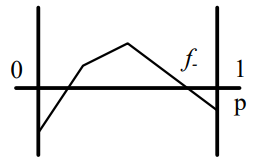
\includegraphics{images/fminus.PNG}
\end{figure}

\noindent
If player 1 wishes to maximize their minimum payoff, then they should choose $p$ such that $f_-(p)$ is maximized.
For this particular example, $p$ can be computed by solving the equation:

\begin{table}[h]
    \centering
    \begin{tabular}{rcll}
    $f_1(p)$ & $=$ & $f_3(p)$ & or written differently: \\
    $4p$ & $=$ & $-6p + 5$ & 
    \end{tabular}
\end{table}

\noindent
This gives $p = \frac{1}{2}$ and $f_1(p) = f_3(p) = 2$.
Thus, by playing the mixed action $(\frac{1}{2}, \frac{1}{2})$, player 1 knows that their expected payoff is going to be at least 2.

\noindent
\\
We now examine the situation from player 2's perspective.
If player 2 uses a mixed action $q = (q_1, q_2, q_3)$ and player 1 plays $T$, then player 1 gets the following expected payoff:
\[ E_1(q) = 0 \cdot q_1 - 2 \cdot q_2 + 5 \cdot q_3 \]

\noindent
If player 1 plays $B$, then player 1 gets the following expected payoff:
\[ E_2(q) = 4 \cdot q_1 + 10 \cdot q_2 - 1 \cdot q_3 \]

\noindent
If player 1 plays the mixed strategy $(1 - p, p)$, then player 1's expected payoff is:
\[ (1 - p) \cdot E_1(q) + p \cdot E_2(q) \]

\noindent
The maximum amount player 2 will have to pay, in expectation, is $\max \{ E_1(q), E_2(q) \}$.

\newpage
\noindent
Player 2 will try to choose their mixed action $q$ in such a way as to keep $\max \{ E_1(q), E_2(q) \}$ as small as possible.
We can visualize the payoff for player 2 as a weighted sum of the separate columns $f_q(p) = q_1 \cdot f_1(p) + q_2 \cdot f_2(p) + q_3 \cdot f_3(p)$: 

\begin{figure}[h]
    \centering
    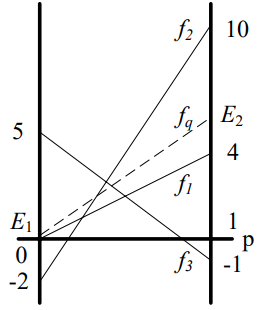
\includegraphics[scale=0.8]{images/fqplot.PNG}
\end{figure}

\noindent
What $q$ should player 2 choose?
We know that player 1 will choose $p = \frac{1}{2}$ because this means that player 1's expected payoff is at least $f_1(\frac{1}{2}) = f_3(\frac{1}{2}) = 2$.
We can also calculate that $f_2(\frac{1}{2}) = 4$.
This means that if player 2 would take $q_2 \neq 0$, then $f_q(\frac{1}{2}) > 2$.
The only way player 2 could be able to make sure that they should never pay more than 2 (in expectation) is by taking $q_2 = 0$, and by taking $q_1$ and $q_3$ such that $E_1(q) = E_2(q) = 2$:

\begin{figure}[h]
    \centering
    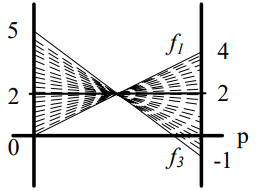
\includegraphics[scale=0.9]{images/f1f3fq.PNG}
\end{figure}

\noindent
To do so, player 2 should balance the graphs of $f_1$ and $f_3$.
To achieve this balance, we need to turn the picture and look at the length of the "arms":

\begin{figure}[h]
    \centering
    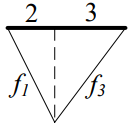
\includegraphics[scale=0.8]{images/f1f3arms.PNG}
\end{figure}

\noindent
This shows that $q_1$ should be $\frac{3}{2}$ times as big as $q_3$.
Thus, by playing the mixed strategy $(\frac{3}{5}, 0, \frac{2}{5})$ player 2 can be sure that the expected payoff to player 1 is not going to be more than 2.

\noindent
\\
If for a matrix game $A$ there are mixed actions $p^* = (p^*_1, p^*_2, ... , p^*_m)$ for player 1 and $q^* = (q^*_1, q^*_2, ... , q^*_n)$ for player 2, and a number $v \in \mathbb{R}$ such that for all mixed actions $p$ and $q$ we have:
\[ p^*Aq \geq v \geq pAq^* \]

\noindent
Then $v$ is called the \textbf{value} of $A$ and mixed actions $p^*, q^*$ are called the \textbf{optimal mixed actions} for player 1 and player 2 respectively.
The \textbf{minimax-theorem} states that every matrix game has a value and that there exist optimal mixed actions for both players.

%
% Topic 3 - Repeated Games
%
\newpage
\section{Repeated Games}
A two-player \textbf{repeated game} consists of a bimatrix game $(A, B)$ that is to be played repeatedly.
At each state $t$ player 1 chooses a row $i$ and player 2 chooses a column $j$.
Immediately player 1 receives payoff $a_{ij}$ and player 2 receives payoff $b_{ij}$, and both players are informed that entry $(i, j)$ was played.
The game then moves to state $t + 1$ where both players have to choose actions again.
In a \textit{finitely} repeated game the set of stages is a finite set $\{ 1, 2, 3, ... , N \}$, while in an \textit{infinitely} repeated game the set of stages is the set of natural numbers $\mathbb{N}$.
In either case both players aim to maximize their average expected payoff, called the \textbf{rewards}, taken over the set of stages.
If $a_t$ is the payoff for player 1 at stage $t$, then player 1's reward is given by:

\begin{table}[h]
    \centering
    \begin{tabular}{rl}
        $\displaystyle \frac{1}{N} \sum_{t = 1}^{N} a_t$ \hspace{1cm} & for finitely repeated games \\
        $\displaystyle \lim_{N \to \infty} \frac{1}{N} \sum_{t = 1}^{N} a_t$ \hspace{1cm} & for infinitely repeated games
    \end{tabular}
\end{table}

\noindent
Consider the following bimatrix game:
\[ \begin{pmatrix}
    2,1 & 0,0 \\
    0,0 & 1,2
\end{pmatrix} \]

\noindent
In a regular game, there does not exist any equilibrium that gives each player an expected payoff of $\frac{3}{2}$.
However, in a repeated game, the players could achieve this by playing the sequence of actions:
\[ (T, L), (B, R), (T, L), (B, R), ... \]

\noindent
The sequence of player 1's actions is a best reply to the sequence of player 2's actions, and vice versa, meaning that this sequence would be an equilibrium in an \textit{infinitely} repeated game.
In a \textit{finitely} repeated game, player 1 could deviate from the sequence in the last stage for their own gain. Player 2, anticipating this deviation, could deviate in the second-to-last stage, and so on.
Therefore this sequence is not an equilibrium in a finitely repeated game.
The set of feasible rewards for this repeated game is shown in the following figure, created by connecting the convex polygon formed by the payoffs of the pure actions:

\begin{figure}[h]
    \centering
    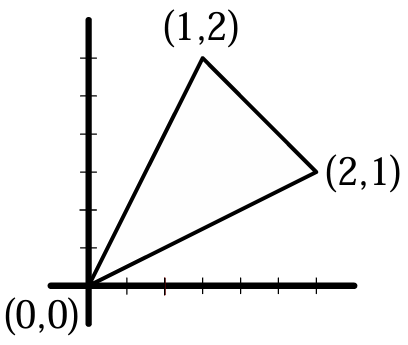
\includegraphics[scale=0.45]{images/feasiblerewards.png}
\end{figure}
\vspace{-0.75cm}

\subsection{Threat Strategies}
In the one-shot version of this game both players can play the mixed equilibrium $\left( \left( \frac{2}{3}, \frac{1}{3} \right), \left( \frac{1}{3}, \frac{2}{3} \right) \right)$, leading to an expected payoff of at least $\frac{2}{3}$ for both players.
This means that both players could also achieve a reward of at least $\frac{2}{3}$ in the repeated game by playing this mixed strategy in every stage.
Consequently, no equilibrium in the repeated game could give a player a reward less than $\frac{2}{3}$.
However, in an infinitely repeated game, the reverse is also true: every feasible reward that gives both players at least $\frac{2}{3}$ can be achieved as an equilibrium!

\newpage
\noindent
Consider the reward $\left( \frac{3}{4}, 1 \right)$.
This reward can be achieved by playing the following sequence of actions:

\[ \left( \frac{3}{4}, 1 \right) = \alpha \cdot (2, 1) + \beta \cdot (1, 2) + (1 - \alpha - \beta) \cdot (0, 0) \]
\[ \big\Downarrow \]
\[ \underbrace{\overbrace{(T, L), (T, L)}^{2}, \overbrace{(B, R), ... , (B, R)}^{5}, \overbrace{(B, L), ... , (B, L)}^{5}}_{12} \]

\noindent
This sequence of actions is not yet an equilibrium, since against the sequence $2 \times L, 5 \times R, 5 \times L$, which is being played by player 2, player 1 could deviate to the sequence $2 \times T, 5 \times B, 5 \times T$ to increase their reward to $\frac{7}{6}$.
However, player 2 would immediately observe that player 1 is deviating, and could therefore respond by deviating to the mixed strategy $\left( \frac{1}{3}, \frac{2}{3} \right)$ for all future stages, giving player 1 a reward of only $\frac{2}{3}$, worse than they would have gotten by sticking to the original sequence.
We can use this idea to incorporate a \textbf{threat} into player 2's strategy $\sigma$:

\begin{enumerate}
    \item Play the sequence $2 \times L, 5 \times R, 5 \times L$.
    \item If player 1 deviates from the sequence $2 \times T, 10 \times B$, then play $\left( \frac{1}{3}, \frac{2}{3} \right)^\infty$ (for all future stages).
\end{enumerate}

\noindent
For player 1 we can define a similar strategy $\pi$:

\begin{enumerate}
    \item Play the sequence $2 \times T, 10 \times B$.
    \item If player 2 deviates from the sequence $2 \times L, 5 \times R, 5 \times L$, then play $\left( \frac{2}{3}, \frac{1}{3} \right)^\infty$.
\end{enumerate}

\noindent
The strategies $\pi$ and $\sigma$ are best replies to each other, and therefore form an equilibrium in the infinitely repeated game.
This equilibrium yields a reward pair of $\left( \frac{3}{4}, 1 \right)$.
Strategies $\pi$ and $\sigma$ are called \textbf{threat strategies}, since they threaten the opponent to stick to the equilibrium sequence.

\noindent
\\
We can generalize the above example for any infinitely repeated game $(A, B)$.
Let $v_A$ and $v_B$ be the matrix game value for player 1 and 2 respectively.
If player 2 is maximizing their payoff while player 1 is minimizing player 2's payoff, then there exist mixed actions $q^\ast$ and $p^\ast$ such that for any $p$ and $q$:
\[ pAq^\ast \leq v_A \quad \text{and} \quad p^\ast Bq \leq v_B \]

\noindent
By using $p^\ast$ player 1 can make sure that player 2 cannot get any reward above $v_B$, and by using $q^\ast$ player 2 can make sure that player 1 can get no reward above $v_A$.
These threat strategies can be applied to any sequence of pure actions that yields a reward pair of at least $(v_A, v_B)$, called the \textbf{threat point}.
All of these concepts are summarized in the \textbf{Folk Theorem}: in an infinitely repeated game, every feasible reward pair above the threat point can be achieved as an equilibrium.

\begin{figure}[h]
    \centering
    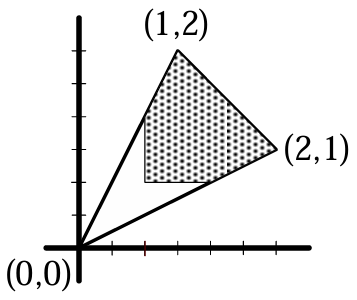
\includegraphics[scale=0.55]{images/folktheorem.png}
\end{figure}

\newpage
\subsection{Repeated Games with Absorbing States}
Repeated games with absorbing states can be represented by a bimatrix where, like before, the entries contain payoffs to the players.
However, now there are some entries marked with an $\ast$. These entries are called \textbf{absorbing states}.
Like in a regular repeated game, the players play the bimatrix game repeatedly, as long as they have not reached an absorbing state.
As soon as an absorbing state with payoffs $(a, b)$ is reached, the game is essentially over. Player 1 and 2 will receive payoffs $a$ and $b$ respectively at all future stages.
If at some stage, no matter when, an absorbing state with payoffs $(a, b)$ is reached, then the average reward for player 1 and 2 will be $(a, b)$ no matter the payoffs in the previous stages.

\noindent
\\
One of the most popular repeated games with absorbing states is the \textbf{Big Match}: a two-player repeated zerosum game with two absorbing states:
\[ \begin{pmatrix}
    1 & 0 \\
    0^\ast & 1^\ast
\end{pmatrix} \]

\noindent
By looking at this matrix, we can make the following observations:

\begin{enumerate}
    \item If player 1 plays a strategy $(1 - p, p)$ at all stages for a fixed $p$, then they cannot be sure of getting any reward greater than $0$. If $p = 0$, then player 1 would get a reward of $0$ if player 2 only plays $R$. If $p > 0$, then an absorbing state will be reached at some stage, giving player 1 a reward of $0$ if player 2 only plays $L$.
    \item If player 1 plays a strategy $(1 - p_t, p_t)$ at stage $t = 1, 2, 3, ...$ for some fixed probabilities $p_1, p_2, p_3, ...$, then they cannot be sure of getting any reward greater than $0$. The argument is similar to the previous observation: If the probability that player 1 ever plays $B$ is $1$, then player 1 will get a reward of $0$ if player 2 only plays $L$. If the probability that player 1 ever plays $B$ is smaller than 1, then for every $\epsilon > 0$ there exists a stage $N_\epsilon$ such that the probability of player 1 ever playing $B$ after stage $N_\epsilon$ will be at most $\epsilon$. This means that player 1's reward will be at most $\epsilon$ if player 2 plays $L$ up to stage $N_\epsilon$, followed by $R$ thereafter.
    \item If player 2 plays $\left( \frac{1}{2}, \frac{1}{2} \right)$ at all stages, then the expected payoff for player 1 is $\frac{1}{2}$, no matter what player 1 plays. If player 2 plays a strategy $(1 - q_t, q_t)$ at stage $t = 1, 2, 3, ...$ for some fixed probabilities $q_1, q_2, q_3, ...$, then there are again two possibilities: If $q_t \leq \frac{1}{2}$ for all $t$, then player 1 can get at least $\frac{1}{2}$ by playing $T$ at all stages. If there exists a stage $t$ such that $q_t > \frac{1}{2}$, then player 1 can get at least $\frac{1}{2}$ by playing $T$ at all stages up to stage $t$, and $B$ thereafter. This means that player 2 can guarantee that player 1's reward will not exceed $\frac{1}{2}$, but they cannot guarantee any lower reward.
    \item Player 1 cannot have a strategy $\pi$ that guarantees a reward of $\frac{1}{2}$. If $\pi$ never chooses $B$ with positive probability, then player 1 will get a reward of $0$ if player 2 plays $R$ at all stages. If $\pi$ does choose $B$ with positive probability, starting at stage $t$, then player 2 could play $L$ at stage $t$, followed by $\left( \frac{1}{2}, \frac{1}{2} \right)$ at all future stages. This means the reward for player 1 for the strategy pair $(\pi, \sigma)$ is:
    \[ (1 - p) \cdot \frac{1}{2} + p \cdot 0 < \frac{1}{2} \]
\end{enumerate}

\noindent
These observations show that player 1 cannot guarantee any reward higher than 0, while player 2 can guarantee that player 1 gets at most $\frac{1}{2}$.
This arises the question: does the Big Match have a value?

\newpage
\noindent
It was eventually proven that player 1 can guarantee a reward of at least $\frac{1}{2} - \frac{1}{N}$ for any non-negative integer $N$ by carefully taking into account the opponent's behavior.
The exact strategy for player 1 to guarantee this reward is to play $B$ at stage $t + 1$ with the following probability:
\[ \frac{1}{(k_t + N + 1)^2} \]

\noindent
Where $k_t = L_t - R_t$ is the number of times player 2 has played $L$ minus the number of times they have played $R$ up to stage $t$. 
This strategy is called an \textbf{$\epsilon$-optimal} strategy for player 1, as it guarantees a reward of at least $\frac{1}{2} - \epsilon$ for any $\epsilon > 0$.

\subsection{\texorpdfstring{$\epsilon$}{epsilon}-Equilibria}
This result can be generalized to show that any zerosum repeated game with absorbing states has a value.
A strategy is said to be a \textbf{Markov strategy} if it only depends on the current state and not on the history of states and actions, and \textbf{stationary} if it is also time-independent.
If a repeated game only contains at most 1 absorbing state per row and column, then there exist stationary ($\epsilon$-)optimal strategies for both players.
See the following examples:
\vspace{-0.5cm}

\begin{multicols}{2}
    \[ \begin{pmatrix}
        1 & 0 \\
        0 & 1^\ast
    \end{pmatrix} \begin{cases}
        v: 1 \\
        \pi: (1 - \epsilon, \epsilon) \\
        \sigma: \text{anything}
    \end{cases} \]

    \[ \begin{pmatrix}
        2^\ast & 0 \\
        0 & 1^\ast
    \end{pmatrix} \begin{cases}
        v: 1 \\
        \pi: (1 - p, p) \text{ where } 0 < p < 1 \\
        \sigma: (0, 1)
    \end{cases} \]
\end{multicols}
\begin{multicols}{2}
    \[ \begin{pmatrix}
        -2 & 6 \\
        5 & 4^\ast
    \end{pmatrix} \begin{cases}
        v: 4 \\
        \pi: (0, 1) \\
        \sigma: (1 - \epsilon, \epsilon)
    \end{cases} \]

    \[ \begin{pmatrix}
        -1 & 3^\ast \\
        4 & -2 \\
        0 & 1
    \end{pmatrix} \begin{cases}
        v: 3 \\
        \pi: (\epsilon, 1 - \epsilon, 0) \\
        \sigma: (0, 1)
    \end{cases} \]
\end{multicols}

\noindent
This theorem also applies to non-zerosum repeated games with absorbing states.
In these games any ($\epsilon$-)equilibrium must achieve a reward greater than or equal to the values of the zerosum games corresponding to the payoffs of the players.
See the following examples:

\begin{multicols}{2}
    \begin{center}
        \begin{tabular}{c|c c}
            $\begin{pmatrix}
                1, 0 & 0, 1 \\
                0, 2 & 1, 0^\ast
            \end{pmatrix}$ & $\pi$ & $\sigma$ \\ \hline
            $v^1 = 1$ & $(1 - \epsilon, \epsilon)$ & anything \\
            $v^2 = 0$ & $(1 - \epsilon, \epsilon)$ & anything \\
            equilibrium: & $((1 - \epsilon, \epsilon),$ & anything$)$
        \end{tabular}
    \end{center}

    \begin{center}
        \begin{tabular}{c|c c}
            $\begin{pmatrix}
                1, 0 & 0, 1^\ast \\
                0, 2^\ast & 1, 0
            \end{pmatrix}$ & $\pi$ & $\sigma$ \\ \hline
            $v^1 = 0$ & anything & $\left( \frac{1}{2}, \frac{1}{2} \right)$ \\
            $v^2 = 1$ & $(1, 0)$ & $\left( \frac{1}{2}, \frac{1}{2} \right)$ \\
            equilibrium: & $((1, 0),$ & $\left( \frac{1}{2}, \frac{1}{2} \right))$
        \end{tabular}
    \end{center}
\end{multicols}
\begin{multicols}{2}
    \begin{center}
        \begin{tabular}{c|c c}
            $\begin{pmatrix}
                3, 1 & 1, 5^\ast \\
                2, 3^\ast & 0, 4
            \end{pmatrix}$ & $\pi$ & $\sigma$ \\ \hline
            $v^1 = 1$ & $(1, 0)$ & $(0, 1)$ \\
            $v^2 = 4$ & $(0, 1)$ & $(0, 1)$ \\
            equilibrium: & $((1, 0),$ & $(0, 1))$
        \end{tabular}
    \end{center}

    \begin{center}
        \begin{tabular}{c|c c}
            $\begin{pmatrix}
                4, 2 & 0, 3^\ast \\
                1, 4^\ast & 4, 0 \\
                2, 1 & 1, 0
            \end{pmatrix}$ & $\pi$ & $\sigma$ \\ \hline
            $v^1 = 1$ & $(0, 1, 0)$ & $(\epsilon, 1 - \epsilon)$ \\
            $v^2 = 1$ & $(0, 0, 1)$ & $(1, 0)$ \\
            equilibrium: & $((0, 1, 0),$ & $(\epsilon, 1 - \epsilon))$
        \end{tabular}
    \end{center}
\end{multicols}

\begin{center}
    \begin{tabular}{c|c c}
        $\begin{pmatrix}
            2, 0 & -2, 8 & 1, -1 \\
            -3, 3^\ast & 2, 4 & 0, 5
        \end{pmatrix}$ & $\pi$ & $\sigma$ \\ \hline
        $v^1 = -2$ & $(1, 0)$ & $(\epsilon, 1 - \epsilon, 0)$ \\
        $v^2 = 4\frac{3}{5}$ & $(\frac{3}{20}, \frac{17}{20})$ & $(0, \frac{3}{5}, \frac{2}{5})$ \\
        equilibrium: & $((1, 0),$ & $(\epsilon, 1 - \epsilon, 0))$
    \end{tabular}
\end{center}

%
% Topic 4 - Stochastic Games
%
\newpage
\section{Stochastic Games}
A two-player \textbf{stochastic game} with finite state and action spaces is defined by a finite set of matrices $A^1, A^2, ... , A^z$ corresponding to the set of states $S = \{ 1, 2, ... , z \}$.
Each matrix $A^s$ can have a unique shape and each entry $(i, j)$ of $A^s$ contains a state-dependent payoff $r^k(s, i, j) \in \mathbb{R}$ for each player $k$, and a transition probability vector $p(s, i, j) = ( p(1|s, i, j), p(2|s, i, j), ... p(z|s, i, j) )$, where $p(t|s, i, j)$ is the probability of transitioning from state $s$ to state $t$ whenever entry $(i, j)$ of $A^s$ is selected.
Play can start in any state $s \in S$ and evolves by players independently choosing actions $i_n$ and $j_n$ at each stage $n$.
A strategy for a player is a rule that tells them for any \textbf{history} of states and actions what (mixed) action to play. If the current state is $s_n$, then the history up until stage $n$ is given by:
\[ h_n = (s_1, i_1, j_1, s_2, i_2, j_2, ... , s_{n-1}, i_{n-1}, j_{n-1}, s_n) \]

\subsection{Discounted Rewards}
For any initial state $s \in S$ and any pair of strategies $(\pi, \sigma)$, the \textbf{limiting average reward} for player $k$ is given by:
\[ \gamma^k(s, \pi, \sigma) = \mathbb{E}_{s\pi\sigma} \left( \liminf_{T \to \infty} \frac{1}{T} \sum_{n = 1}^{T} r^k(S_n, I_n, J_n) \right) \]

\noindent
Where $S_n, I_n, J_n$ are random variables for the state and actions at stage $n$.
Similarly, the \textbf{$\beta$-discounted reward} for $\beta \in (0, 1)$ is given by:
\[ \gamma^k_\beta(s, \pi, \sigma) = \mathbb{E}_{s\pi\sigma} \left( (1 - \beta) \sum_{n = 1}^{\infty} \beta^{n-1} r^k(S_n, I_n, J_n) \right) \]

\noindent
For example, suppose that the sequence of payoffs is $1, 1, 1, 1, 1, 1, 1, 1, ...$.
The limiting average reward is $1$, and for any $\beta \in (0, 1)$ the $\beta$-discounted reward is:
\[ (1 - \beta)\left( 1 + \beta + \beta^2 + \beta^3 + ... \right) = \frac{(1 - \beta)}{(1 - \beta)} = 1 \]

\noindent
If the sequence of payoffs results from jumping back and forth between two states where the payoffs are 1 and 2 respectively, then the limiting average reward will be $\frac{3}{2}$, while the $\beta$-discounted reward for the different initial states will be:
\begin{align*}
    \gamma_\beta(1) &= (1 - \beta)\left( 1 + 2\beta + \beta^2 + 2\beta^3 + \beta^4 + 2\beta^5 + ... \right) \\
    \gamma_\beta(2) &= (1 - \beta)\left( 2 + \beta + 2\beta^2 + \beta^3 + 2\beta^4 + \beta^5 + ... \right)
\end{align*}

\noindent
Though it is not immediately obvious what these expressions accumulate to, notice that $\gamma_\beta(1) = (1 - \beta) + \beta\gamma_\beta(2)$ and $\gamma_\beta(2) = 2(1 - \beta) + \beta\gamma_\beta(1)$.
From these equations we can calculate the $\beta$-discounted rewards for both initial states:
\[ \gamma_\beta(1) = \frac{1 + 2\beta}{1 + \beta} \quad \quad \gamma_\beta(2) = \frac{2 + \beta}{1 + \beta} \]

\noindent
The limiting average reward $\gamma^k(x, y)$ and the $\beta$-discounted reward $\gamma^k_\beta(x, y)$ for stationary strategies $(x, y)$ are related by the following formula:
\[ \gamma^k(x, y) = \lim_{\beta \uparrow 1} \gamma^k_\beta(x, y) \]

\newpage
\noindent
A \textbf{$k$-zerosum game} is a stochastic game where player $k$ is maximizing their reward while the other player is minimizing player $k$'s reward.
It can be shown that for any $k$-zerosum game with any $\beta \in (0, 1)$, there exists a $\beta$-discounted value $v_\beta^k$ and a pair of stationary $\beta$-discounted optimal strategies $(x_\beta^k, y_\beta^k)$.
These optimal strategies can be created to be independent of the initial state $s$.

\noindent
\\
Stochastic games where the only non-zero payoffs can be achieved in absorbing states are called \textbf{recursive games}.
For these games it can be shown that there exists a limiting average value $v^k$, which can be achieved through a pair of stationary $\epsilon$-optimal strategies $(x_\epsilon^k, y_\epsilon^k)$.
The limiting average value $v^k$ actually exists for any stochastic game, although in most games this value can only be achieved through history-dependent strategies.
For general-sum stochastic games, it can be shown that stationary $\beta$-discounted equilibria exist.
However, limiting average $\epsilon$-equilibria are only guaranteed to exist in two-player games.

\subsection{Markov Decision Processes}
A stationary strategy $x$ is called \textbf{pure} if $x_s$ is a pure action for all states $s$.
Notice that if one player plays a stationary strategy while the opponent knows this strategy, then the opponent is essentially facing a Markov decision problem.
Since pure stationary optimal strategies exist for Markov decision problems with finite state and action spaces, it follows that, when playing against a fixed stationary strategy, a player always has a pure stationary best reply $f^k$.
However, this is difficult to achieve in general stochastic games, as the opponent's strategy is not known in advance.
Even stochastic games with perfect information do not admit stationary $\epsilon$-equilibria in general.
Consider the following example:

\begin{figure}[h]
    \centering
    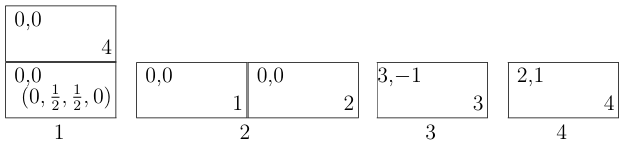
\includegraphics{images/stochastic1.PNG}
\end{figure}

\noindent
This is a two-player stochastic game with four states, where player 1 has two actions in state 1, player 2 has two actions in state 2, and state 3 and 4 are absorbing states.
The numbers in the top left corner of each state-action pair represent the immediate payoffs for both players, while the numbers in the bottom right corners represent the transition function.

\noindent
\\
Suppose player 2 always plays $R$ in state 2, which gives both players a reward of 0.
A best reply for player 1 to this strategy is to always play $T$ in state 1, as that would give player 1 a reward of 2 instead of the expected reward of $\frac{3}{2}$ they would get by playing $B$.
Player 2, anticipating this, could benefit by putting some positive probability on $L$ in state 2, as this would give player 2 a reward of 1 instead of 0.
However, player 1 could then put some positive probability on $B$ in state 1, as state 2 is now no longer an absorbing state.
This puts player 2 at risk of getting a reward of -1, which is worse than the reward of 0 they would get by only playing $R$.
This shows that there exists no stationary ($\epsilon$-)equilibrium for this game.
However, there do exist non-stationary equilibria for this game:

\[ \left( T, L \text{ with threat to play } R \right) \]
\[ \left( T \text{ with threat to play } B, R \right) \]

\newpage
\noindent
We can find general non-stationary equilibria for perfect information stochastic games through the following procedure:

\begin{enumerate}
    \item Take a pure stationary limiting average optimal strategy $f^1$ for player 1 (e.g. $f^1 = T$).
    \item Let $g^1$ be a pure stationary limiting average optimal strategy for player 2 in the 1-zerosum game against $f^1$ (e.g. $g^1 = R$).
    \item Let $g^2$ be a pure stationary limiting average best reply for player 2 against $f^1$ in the 2-zerosum game (e.g. $g^2 = L$).
    \item Define $g^\ast$ for player 2 as: play $g^2$ unless at some stage player 1 deviates from playing $f^1$, in which case play $g^1$.
\end{enumerate}

\noindent
From this it can be shown that $(f^1, g^\ast)$ is a limiting average equilibrium.
We can also find a $\beta$-discounted equilibrium for this game 
by solving the following equations:
\[ \gamma^1_{1 \beta T} = \gamma^1_{1 \beta B} \quad \quad \gamma^2_{2 \beta L} = \gamma^2_{2 \beta R} \]

\noindent
Where $\gamma^k_{s \beta a}$ is the $\beta$-discounted reward for player $k$ when playing $a$ starting in state $s$:

\[ \gamma^k_{s \beta a} = (1 - \beta) r^k(s, a) + \beta \sum_{s^\prime} P(s^\prime | s, a) \gamma^k_{s^\prime \beta a} \]

\noindent
First of all, observe that $\gamma^2_{2 \beta R}$ should be equal to 0:

\[ \gamma^2_{2 \beta L} = 0 \cdot (1 - \beta) + \beta \gamma^2_{1 \beta L} = \underbrace{\gamma^2_{2 \beta R}}_{=0} \Longrightarrow \gamma^2_{1 \beta L} = 0 \]
\[ \underbrace{\gamma^2_{1 \beta L}}_{=0} = 0 \cdot (1 - \beta) + \beta (1 - p) \underbrace{\gamma^2_{4 \beta L}}_{=1} + \frac{1}{2} \beta p \underbrace{\gamma^2_{2 \beta L}}_{=0} + \frac{1}{2} \beta p \underbrace{\gamma^2_{3 \beta L}}_{=-1} \]
\[ \beta (1 - p) - \frac{1}{2} \beta p = 0 \Longrightarrow p = \frac{2}{3} \]

\noindent
Where $p$ is the probability of player 1 playing $B$ in state 1.
Similarly, we can find $q$, the probability of player 2 playing $R$ in state 2, by observing that $\gamma^1_{1 \beta T}$ should be equal to $2\beta$:

\[ \underbrace{\gamma^1_{1 \beta T}}_{=2\beta} = \gamma^1_{1 \beta B} = 0 \cdot (1 - \beta) + \frac{1}{2} \beta \gamma^1_{2 \beta B} + \frac{1}{2} \beta \underbrace{\gamma^1_{3 \beta B}}_{=3} \Longrightarrow \gamma^1_{2 \beta B} = 1 \]
\[ \underbrace{\gamma^1_{2 \beta B}}_{=1} = 0 \cdot (1 - \beta) + \beta (1 - q) \underbrace{\gamma^1_{1 \beta B}}_{=2\beta} + \beta q \underbrace{\gamma^1_{2 \beta B}}_{=1} \]
\[ 2\beta^2(1 - q) + \beta q = 1 \Longrightarrow q = \frac{2\beta^2 - 1}{2\beta^2 - \beta} \]

\noindent
This means we have the following $\beta$-discounted equilibrium:

\[ \left( \left( \frac{1}{3}, \frac{2}{3} \right), \left( \frac{1 - \beta}{2\beta^2 - \beta}, \frac{2\beta^2 - 1}{2\beta^2 - \beta} \right) \right) \]

%
% Topic 5 - Games in Extensive Form
%
\newpage
\section{Games in Extensive Form}
A \textbf{perfect information game} is a game where every possible situation (the past history and all possible future developments) is known to all players.
So far we have only worked with \textbf{stategic form games}, where the players simultaneously choose their actions.
In \textbf{extensive form games} the game is represented as a tree, which allows for the explicit representation of the sequencing of players' possible moves and their choices at each decision point.
Consider the following example:

\begin{figure}[h]
    \begin{minipage}[h]{.6\linewidth}
        \centering
        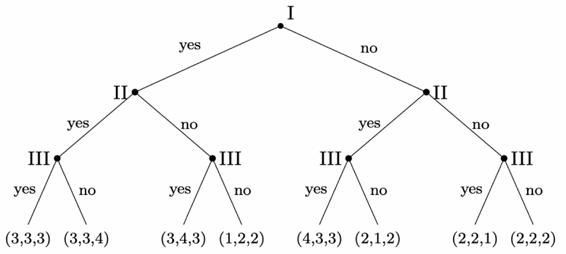
\includegraphics[scale=0.7]{images/extensiveform-ex1.PNG}
    \end{minipage}\hfill
    \begin{minipage}[h]{.4\linewidth}
        \centering
        \begin{tabular}{cc|c}
            \textbf{vote} & \textbf{raise} & \textbf{utility} \\ \hline
            no & yes & 4 \\
            yes & yes & 3 \\
            no & no & 2 \\
            yes & no & 1
        \end{tabular}
    \end{minipage}
\end{figure}

\noindent
This is a game where three politicians must vote to raise or not raise their salaries.
This voting is done in public and in sequence, so each politician knows the previous votes before making their own.
For each politician their preferred outcome is to have their salaries raised, but in the public eye it is better to vote against the raise.

\subsection{Backwards Induction}
The rational outcomes of a finite, perfect information game can be found through a procedure known as \textbf{backwards induction}.
Starting at the left-most pair of leaves, we can determine that the third politician will vote against the raise, as this will give them a utility of 4 instead of 3.
In the second pair of leaves, the third politician will vote in favor of the raise, as this will give them a utility of 3 instead of 2.
The second politician, knowing this, will vote against the raise in the left branch, as this will give them a utility of 4 instead of 3.
By repeating this process we eventually find that the first politician will vote against the raise, while the second and third politicians will vote in favor of the raise, resulting in a utility of $(4, 3, 3)$.

\noindent
\\
Given a perfect information game in extensive form, a \textbf{strategy} for a player is a complete specification of what action to take at each decision point.
A \textbf{strategy profile} is a tuple of strategies, one for each player.
See the following example:

\begin{figure}[h]
    \begin{minipage}[h]{.5\linewidth}
        \centering
        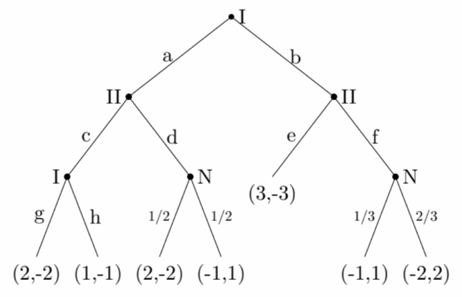
\includegraphics[scale=0.7]{images/extensiveform-ex2.PNG}
    \end{minipage}\hfill
    \begin{minipage}[h]{.5\linewidth}
        \centering
        \begin{align*}
            \text{strategies I: } & \{ ag, ah, bg, bh \} \\
            \text{strategies II: } & \{ ce, cf, de, df \} \\
            \text{expected outcome: } & (\frac{1}{2}, -\frac{1}{2}) \\
            \text{optimal strategies: } & (ag, df)
        \end{align*}
    \end{minipage}
\end{figure}

\noindent
This is an example of a stochastic game in extensive form.
In stochastic games a random outcome is denoted by an $N$ node, where $N$ stands for nature.

\newpage
\subsection{Strategic Form}
Consider the following game in strategic form:

\[ \begin{pmatrix}
    1, 2 & 1, 3 \\
    0, 2 & a, b
\end{pmatrix} \]

\noindent
The rows in this matrix correspond to the strategies of player 1, while the columns correspond to the strategies of player 2.
This means that this game in extensive form must have two strategies (i.e. branches) for both player 1 and 2.
The only way to draw a tree for this game is to have an action of one player lead to the decision node of the other player.
Therefore, the only way for this game to be representable in extensive form is for $(a, b)$ to equal $(0, 2)$ if player 1 starts, or $(1, 3)$ if player 2 starts:

\begin{multicols}{2}
    \Tree[.I [.II 1,2 1,3 ] [ 0,2 ] ]

    \Tree[.II [.I 1,2 0,2 ] [ 1,3 ] ]
\end{multicols}

\noindent
Conversion from extensive form to strategic form is also possible, although it comes with the loss of information about the sequence of moves.
The set of strategies for a player in the extensive form game is the set of pure strategies for that player in the strategic form game.
See the following example:

\begin{figure}[h]
    \begin{minipage}[h]{.5\linewidth}
        \centering
        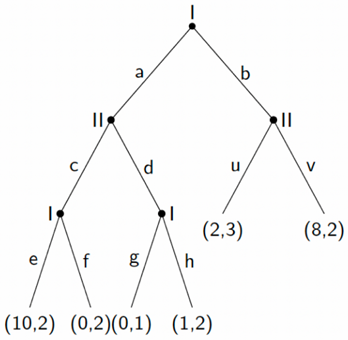
\includegraphics[scale=0.7]{images/extensive-to-strategic.PNG}
    \end{minipage}\hfill
    \begin{minipage}[h]{.5\linewidth}
        \centering
        \begin{tabular}{c|cccc}
            & $cu$ & $cv$ & $du$ & $dv$ \\ \hline
            $aeg$ & $10,2$ & $10,2$ & $0,1$ & $0,1$ \\
            $aeh$ & $10,2$ & $10,2$ & $1,2$ & $1,2$ \\
            $afg$ & $0,2$ & $0,2$ & $0,1$ & $0,1$ \\
            $afh$ & $0,2$ & $0,2$ & $1,2$ & $1,2$ \\
            $beg$ & $2,3$ & $8,2$ & $2,3$ & $8,2$ \\
            $beh$ & $2,3$ & $8,2$ & $2,3$ & $8,2$ \\
            $bfg$ & $2,3$ & $8,2$ & $2,3$ & $8,2$ \\
            $bfh$ & $2,3$ & $8,2$ & $2,3$ & $8,2$
        \end{tabular}
    \end{minipage}
\end{figure}

\noindent
A way to convert a strategic form game to an extensive form game without having to introduce sequential moves is to turn the game into \textbf{imperfect information}.
In imperfect information games we can represent the fact that a player does not know what branch the game is in by using dashed lines:

\begin{figure}[h]
    \centering
    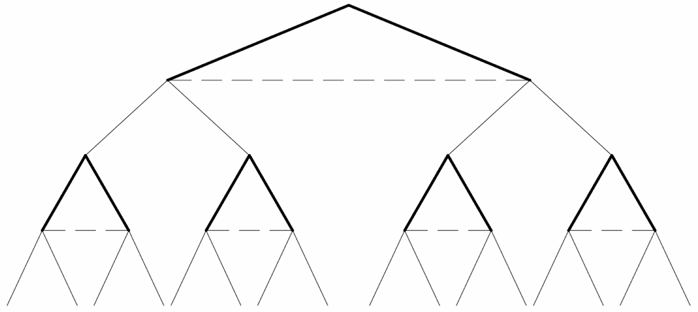
\includegraphics[scale=0.5]{images/imperfectinformationtree.PNG}
\end{figure}

\noindent
The concept of imperfect information can mathematically be represented using \textbf{information sets}.
An information set is a set of decision nodes that are indistinguishable to a player.
The actions available in an information set are the same for all nodes in that set, since otherwise the player would be able to distinguish between the nodes.
Consider the following example:

\newpage
\begin{figure}[h]
    \centering
    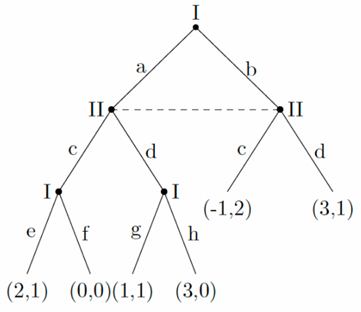
\includegraphics[scale=0.7]{images/imperfectinformation-ex.PNG}
\end{figure}

\noindent
In this game player 1 has the strategies $\{ aeg, aeh, afg, afh, beg, beh, bfg, bfh \}$ and player 2 has the strategies $\{ c, d \}$.
In both of player 2's decision nodes, player 2 does not know what player 1 has played.
This means that player 2 has an information set containing both decision nodes.

\noindent
\\
Note that the equilibrium for a strategic form game is not necessarily an equilibrium for the corresponding extensive form game.
Consider the following game in both strategic and extensive form:

\begin{minipage}[h]{.5\linewidth}
    \[ \begin{pmatrix}
        1, 3 & 1, 3 \\
        0, 0 & 2, 2
    \end{pmatrix} \]
\end{minipage}%
\begin{minipage}[h]{.4\linewidth}
    \Tree[.I [ 1,3 ] [.II 0,0 2,2 ] ]
\end{minipage}

\noindent
The equilibrium $(T, L)$ is not achieved through backwards induction, because it prescribes the non-optimal action $L$ for player 2 in their only decision node.
Additionally, $L$ is also a \textbf{weakly dominated strategy} for player 2.
However, since player 2 only chooses their action after player 1 has chosen theirs, player 2 can threaten to play $L$ if player 1 plays $B$.
This example shows that the concept of Nash-equilibria is based on the strategic form of a game.

\noindent
\\
When applied to a game tree, the strategy profile for all players is assumed to be chosen before the game starts.
The moves in a strategy profile should be optimal for any part of the game, even the parts that are never reached (e.g. the above example where, if player 2 threatens to play $L$, player 2's decision node will never be reached).
A strategy profile that defines a Nash-equilibrium for every \textbf{subgame} (any subtree of the game) is called a \textbf{subgame perfect Nash-equilibrium} (SPNE).

\subsection{Stackelberg Games}
Consider the following game in matrix form:

\[ \begin{pmatrix}
    0, 0 & 3, 1 \\
    1, 3 & 4, 2
\end{pmatrix} \]

\noindent
If players 1 and 2 both have to choose their actions simultaneously, then there is a Nash-equilibrium at $(B, L)$.
However, if player 1 gets to choose their action first, then they can pin player 2 by playing $T$, resulting in an equilibrium at $(T, R)$.
In this scenario where player 1 gets to choose their action first, they are able to claim a higher reward for themselves.
We say that $T$ is the \textbf{Stackelberg strategy} for player 1 (the \textbf{leader}), leading to the \textbf{Stackelberg solution} $(T, R)$ with \textbf{Stackelberg (equilibrium) outcome} $(3, 1)$.
Observe the following example:

\[ \begin{pmatrix}
    0, 0 & -1, 0 & -3, -1 \\
    -2, 1 & -2, 0 & 1, 0
\end{pmatrix} \]

\newpage
\noindent
If player 1 plays $T$, then player 2 is indifferent between playing $L$ and $M$.
In this case player 1 is only able to guarantee a reward of -1. We cannot find a Stackelberg equilibrium for this game, but we can conclude that $T$ is the Stackelberg strategy for player 1.
Now consider the following game:

\[ \begin{pmatrix}
    2, 2 & 1, 0 \\
    3, 1 & 0, 1
\end{pmatrix} \]

\noindent
This game has a Nash-equilibrium at $(B, L)$, and a Stackelberg equilibrium at $(T, L)$ with player 1 as the leader.
The interesting result here is that player 1 is worse off in the Stackelberg equilibrium than in the Nash-equilibrium, despite being the leader.
For a given two-player finite game, let $f_S$ and $f_N$ denote player 1's Stackelberg and Nash payoffs respectively.
If player 2 has a unique best reply for every action of player 1, then $f_S \geq f_N$.

\subsection{Continuous Games}
So far we have only considered games with a finite number of actions.
Consider a game where players 1 and 2 choose numbers $x, y \in \mathbb{R}$.
The cost functions $f, g$ for players 1 and 2 respectively are given by:
\[ f(x, y) = (y-5)^2 + x^2 \qquad \qquad g(x, y) = x^2 + y^2 - xy \]

\noindent
We can find the best replies for both players by finding the minimum of their respective cost functions:
\begin{alignat*}{4}
    \frac{\partial f}{\partial x} = 0 &\ \rightarrow\ 2x &&= 0 &&\ \rightarrow\ x^* = 0, \quad &\frac{\partial^2 f}{\partial x^2} > 0 \\
    \frac{\partial g}{\partial y} = 0 &\ \rightarrow\ 2y - x &&= 0 &&\ \rightarrow\ y^* = \frac{1}{2}x, \quad &\frac{\partial^2 g}{\partial y^2} > 0
\end{alignat*}

\noindent
The Nash-equilibrium lies at the intersection of the best replies, which in this case is $(0, 0)$.
To calculate the Stackelberg equilibrium, the leader minimizes their cost function while considering the best reply of the follower:
\[ \frac{\partial f(x, y^*)}{\partial x} = 0, \quad \frac{\partial^2 f(x, y^*)}{\partial x^2} > 0 \]

\noindent
This results in the Stackelberg strategy $x_S = 2$ for player 1, leading to the Stackelberg equilibrium $(2, 1)$ with a cost of $(f(2, 1)=20, g(2, 1)=3)$, which is better than the Nash-equilibrium $(0, 0)$ with a cost of $(f(0, 0)=25, g(0, 0)=0)$.

%
% Topic 6 - Evolutionary Games
%
\newpage
\section{Evolutionary Games}
In evolutionary games the strategies of the players are not chosen by the players themselves, but inherited from generation to generation.
The heritable traits of players (commonly called \textbf{organisms} in the context of evolutionary games) determine their observable characteristics (strategies) and payoffs (commonly called \textbf{fitness}) in a given environment.
Organisms that are more fit will tend to produce more offspring, meaning that their traits will be passed on to more organisms over time.
A very simple example of an evolutionary game is the \textbf{hawk-dove game}:

\[ \begin{blockarray}{ccc}
    & \text{Hawk} & \text{Dove} \\[1ex]
    \begin{block}{r(cc)}
        \text{Hawk } & \displaystyle \frac{V - C}{2}, \frac{V - C}{2} & V, 0 \\
        \text{Dove } & 0, V & \displaystyle \frac{V}{2}, \frac{V}{2} \\
    \end{block}
\end{blockarray} \]

\noindent
In this game two organisms are contesting over a shared resource of value $V$.
If both organisms are a hawk, they will fight over the resource, resulting in a cost of $C > V$ for both.
If both organisms are a dove, they will share the resource, resulting in a benefit of $\frac{V}{2}$ for both.
If one organism is a hawk and the other is a dove, the hawk will get all of the resource, while the dove will get nothing.

\subsection{Evolutionary Stable Strategies}
In evolutionary games we are interested in finding strategies that, if adopted by a population, cannot be invaded by any other strategy.
These strategies are called \textbf{evolutionary stable strategies} (ESS).
Once an ESS has been established in a population, it will remain in that population indefinitely.
Consider the following variation of the hawk-dove game:

\[ \begin{blockarray}{ccc}
    & \text{Small} & \text{Large} \\[0.5ex]
    \begin{block}{r(cc)}
        \text{Small } & 5, 5 & 1, 8 \\
        \text{Large } & 8, 1 & 3, 3 \\
    \end{block}
\end{blockarray} \]

\noindent
In this game small and large organisms are contesting over food.
When organisms of the same size compete they will get equal shares of food, but when a large organism competes with a small organism the large organism will get the majority of the food.
In general, large organisms experience less of a benefit from a given quantity of food as they require more food to sustain themselves.

\noindent
\\
Imagine that an alternative strategy $t$ tries to invade a population consisting of organisms playing strategy $s$ (i.e. an $\epsilon$-fraction of the population uses $t$ while a $(1 - \epsilon)$-fraction of the population uses $s$).
Suppose that strategy $s$ is equivalent to "Small", while strategy $t$ is equivalent to "Large".
The expected payoff for a small organism in this population is $5 (1 - \epsilon) + 1\epsilon = 5 - 4\epsilon$, while the expected payoff for a large organism is $8(1 - \epsilon) + 3\epsilon = 8 - 5\epsilon$.
From this we can conclude that "Small" is not an evolutionary stable strategy for this game (only for $\epsilon > 3$, which is not possible).

\noindent
\\
To check if "Large" is an ESS, we simply swap the roles of the strategies and repeat the calculations.
The expected payoff for a small organism is $(1 - \epsilon) + 5\epsilon = 1 + 4\epsilon$, while the expected payoff for a large organism is $3(1 - \epsilon) + 8\epsilon = 3 + 5\epsilon$.
In this case we can conclude that "Large" is an ESS for all values of $\epsilon$.
In this example the ESS turned out to be a pure strategy, but an ESS can also be a mixed strategy (e.g. the 1:1 gender ratio in humans is an ESS).

\newpage
\noindent
Another example of an evolutionary game is the \textbf{Prisoner's Dilemma}, a special case of the hawk-dove game when $V > C$.
Similarly to the Nash-equilibrium, the ESS for the Prisoner's Dilemma is $(D, D)$.
This shows us that evolution can be inefficient, as the ESS is not the optimal outcome for the population as a whole.
In general, a dominated strategy (e.g. $C$ in the Prisoner's Dilemma) can never be part of an ESS.
If a strategy is an ESS, then it is also a Nash-equilibrium in the strategic form of the game.
However, being an ESS is a stronger condition than being a Nash-equilibrium, so the opposite is not necessarily true.

\subsection{Mixed Evolutionary Stable Strategies}
A \textbf{monomorphic population} is a population where all organisms have the same strategy, while a \textbf{polymorphic population} is a population where multiple strategies are present.
In the hawk-dove game, neither hawk nor dove is an ESS.
No monomorphic population is possible, as there always exists a best reply that can invade the population.
Consider the following game:

\[ \begin{blockarray}{ccc}
    & \text{Hawk} & \text{Dove} \\[0.5ex]
    \begin{block}{r(cc)}
        \text{Hawk } & -5,-5 & 10,0 \\
        \text{Dove } & 0,10 & 5,5 \\
    \end{block}
\end{blockarray} \]

\noindent
Suppose that some fraction of the population $p$ is a hawk, while the remaining fraction $1 - p$ is a dove.
The expected payoff for a hawk in this population is $-5p + 10(1 - p) = 10 - 15p$, while the expected payoff for a dove is $0p + 5(1 - p) = 5 - 5p$.
The population will be stable if and only if the expected payoff for a hawk is equal to the expected payoff for a dove:
\begin{align*}
    E(\text{Hawk}) &= E(\text{Dove}) \\
    10 - 15p &= 5 - 5p \\
    p^* &= \frac{1}{2}
\end{align*}

\noindent
This means that the ESS for this game is a polymorphic population with half of the organisms being hawks and the other half being doves (for hawk-dove games in general, $p^*_{\text{Hawk}} = \frac{V}{C}$).

\noindent
\\
Let $A$ be a fitness matrix for a population consisting of $n$ strategies, and let $x = (x_1, x_2, ... , x_n)$ be a population distribution over all strategies.
$x$ is an ESS if the following conditions are met:

\begin{enumerate}
    \item $xAx \geq yAx$ for all $y$. None of the other strategies should be able to achieve a higher fitness than $x$ ($x$ is a Nash-equilibrium).
    \item If $yAx = xAx$, then $xAy > yAy$ for all $y \neq x$. If at some point in time the population distribution is $y \neq x$, then over time the population will strictly shift towards $x$.
\end{enumerate}

\noindent
These conditions are automatically satisfied for pure strategies, but need to be verified for mixed strategies.
A useful theorem for finding possible mixed ESS is the \textbf{Bishops-Cannings theorem}:

\begin{enumerate}
    \item All strategies used in a mixed ESS with positive probability must have the same payoff.
    \item None of the strategies used in a mixed ESS with positive probability can be part of a pure ESS.
\end{enumerate}

\noindent
A corollary of this theorem is that if $x$ is a completely mixed ESS (i.e. every strategy is played with positive probability), then $x$ is the only ESS in the game.
Flipping this around, if we find any pure strategy ESS or any non-completely mixed ESS, then there does not exist any completely mixed ESS in the game.
Consider the following example:

\newpage
\[ \begin{pmatrix}
    6,6 & 0,0 & 0,0 \\
    0,0 & 2,2 & 3,5 \\
    0,0 & 5,3 & 2,2
\end{pmatrix} \]

\noindent
Notice that $(1, 0, 0)$ is a pure ESS for this game.
This means that there does not exist a completely mixed ESS for this game, nor a mixed ESS where the first strategy is played with positive probability.
This means that the only other candidate for an ESS is the mixed strategy $(0, p, 1 - p)$:
\[ \begin{blockarray}{cc}
    p & 1 - p \\[0.5ex]
    \begin{block}{(cc)}
        2,2 & 3,5 \\
        5,3 & 2,2 \\
    \end{block}
\end{blockarray} \] \vspace{-1cm}
\begin{align*}
    2p + 3(1 - p) &= 5p + 2(1 - p) \\
    p^* &= \frac{1}{4}
\end{align*}

\noindent
Now that we have a candidate ESS $(0, \frac{1}{4}, \frac{3}{4})$, we need to verify the ESS conditions:

\begin{enumerate}
    \item First we need to check if $(0, \frac{1}{4}, \frac{3}{4})$ is a Nash-equilibrium in mixed strategies:
    \begin{alignat*}{3}
        T &\rightarrow 6 \cdot 0 + 0 \cdot \frac{1}{4} + 0 \cdot \frac{3}{4} &&= 0 \\
        M &\rightarrow 0 \cdot 0 + 2 \cdot \frac{1}{4} + 3 \cdot \frac{3}{4} &&= \frac{11}{4} \\
        B &\rightarrow 0 \cdot 0 + 5 \cdot \frac{1}{4} + 2 \cdot \frac{3}{4} &&= \frac{11}{4}
    \end{alignat*}
    By the B-C theorem, $E(M) = E(B)$. $\frac{11}{4} > E(T) = 0$, so $(0, \frac{1}{4}, \frac{3}{4})$ is a Nash-equilibrium.
    \item Next we need to verify that $(0, \frac{1}{4}, \frac{3}{4})$ is an ESS:
    \begin{align*} \begin{pmatrix}
        0 & \frac{1}{4} & \frac{3}{4}
    \end{pmatrix} \begin{pmatrix}
        6 & 0 & 0 \\
        0 & 2 & 3 \\
        0 & 5 & 2
    \end{pmatrix} \begin{pmatrix}
        0 \\ y \\ 1- y
    \end{pmatrix} &> \begin{pmatrix}
        0 & y & 1 - y
    \end{pmatrix} \begin{pmatrix}
        6 & 0 & 0 \\
        0 & 2 & 3 \\
        0 & 5 & 2
    \end{pmatrix} \begin{pmatrix}
        0 \\ y \\ 1- y
    \end{pmatrix} \\
    &\ \vdots \\
    \left( y - \frac{1}{4} \right)^2 &> 0
    \end{align*}
    This inequality holds for all $y \neq \frac{1}{4}$, so $(0, \frac{1}{4}, \frac{3}{4})$ is an ESS.
\end{enumerate}

\subsection{Population Dynamics}
So far we have assumed that the population distribution $x$ is fixed, but in reality the population can evolve and each component of the population distribution $x$ varies in time:

\[ x(t) = \{ x_i(t) \} \]

\newpage
\noindent
A common model for the evolution of a population distribution is the \textbf{replicator equation}:
\[ \dot{x}_i = x_i \left[ (Ax)_i - xAx \right] \]

\noindent
This equation says that the change in the population distribution of a strategy $\dot{x}_i$ is proportional to the difference between the fitness of that strategy $(Ax)_i$ and the average fitness of the population $xAx$.
The solution to this equation is given by the set of evolutionary stable states of the population.
We can find these states by solving for $\dot{x}_i = 0$, see the following example:

\[ \begin{pmatrix}
    5,5 & 0,2 \\
    2,0 & 2,2
\end{pmatrix} \]

\noindent
Let $p$ be the fraction of the population playing the top strategy.
The expected value of the top strategy is $5p$, while the expected value of the bottom strategy is $2p + 2(1 - p) = 2$.
The average fitness of the population is $5p^2 + 2(1 - p)$.
Since we set the fraction of the top strategy to be $p$, the difference in fitness is $5p - (5p^2 + 2(1 - p)) = -5p^2 + 7p - 2$.
We can find the stable states by solving the following equation:
\begin{align*}
    \dot{x}_i &= 0 \\
    p(-5p^2 + 7p - 2)) &= 0
\end{align*}
\[ \vdots \]
\[ p = 0 \lor p = 1 \lor p = \frac{2}{5} \]

\noindent
Solutions to the replicator equation may or not be \textbf{dynamically stable}.
A solution is dynamically stable if the population will converge to this solution if it is close enough to it.
To see if the population will converge to a solution, we can plot the replicator function $\dot{x}_i$ for $p$:

\begin{figure}[h]
    \centering
    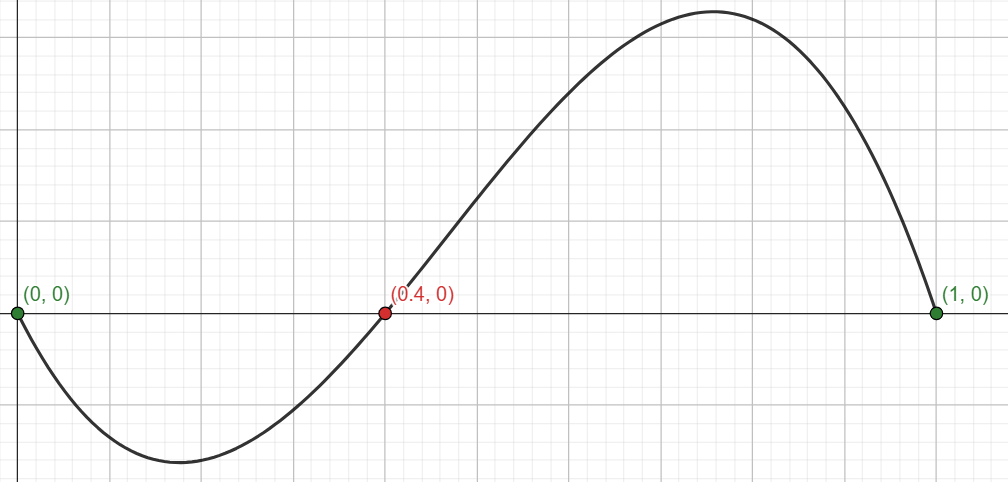
\includegraphics[scale=0.5]{images/derivative.PNG}
\end{figure}

\noindent
If the replicator function is positive, then the population is increasing, meaning the population will shift to a larger $p$.
If the replicator function is negative, then the population is decreasing, meaning the population will shift to a smaller $p$.
In the above example, $p = 0$ and $p = 1$ are both dynamically stable, as the population will gradually shift towards these points.
$p = \frac{2}{5}$ is not dynamically stable, as the population will drift away as soon as it is only slightly off this point.
If the steady points of the replicator equation are dynamically stable, then they are also a Nash-equilibrium.
However, the opposite is not necessarily true.

\end{document}
